\documentclass[xcolor=dvipsnames]{beamer} 
\usetheme{Boadilla}

\usecolortheme{orchid}

\usepackage{multirow}
\usepackage{makecell}
\usepackage{booktabs}
\usepackage{subcaption}

\usepackage{lmodern}
\usepackage[absolute,overlay]{textpos}
\usepackage{graphicx}

\usepackage{mathtools}

\usepackage{xcolor}

\usepackage{soul}

\usepackage{systeme}


%--------RODAPE----------------
\makeatother
\setbeamertemplate{footline}
{
	\leavevmode%
	\hbox{%
		\begin{beamercolorbox}[wd=.33\paperwidth,ht=2.25ex,dp=1ex,center]{author in head/foot}%
			\usebeamerfont{author in head/foot}\insertshortauthor
		\end{beamercolorbox}%
		\begin{beamercolorbox}[wd=.6\paperwidth,ht=2.25ex,dp=1ex,center]{title in head/foot}%
			\usebeamerfont{title in head/foot}\insertshorttitle
	\end{beamercolorbox}}%
	\begin{beamercolorbox}[wd=.07\paperwidth,ht=2.25ex,dp=1ex,center]{author in head/foot}%
		\insertframenumber{} / \inserttotalframenumber\hspace*{0ex}
\end{beamercolorbox}}%
\vskip0pt%
\makeatletter
\setbeamertemplate{navigation symbols}{}


%Backup Slides Command
\newcommand{\backupbegin}{
	\newcounter{finalframe}
	\setcounter{finalframe}{\value{framenumber}}
}
\newcommand{\backupend}{
	\setcounter{framenumber}{\value{finalframe}}
}


%References
\setbeamertemplate{bibliography item}{\insertbiblabel}
\usepackage[backend=biber, bibencoding=utf8, style=ieee, style=authoryear-comp, maxnames=3, natbib, maxbibnames=99]{biblatex}

\usepackage{filecontents}
\begin{filecontents*}{\jobname.bib}
	
%@article{gupta1996bayesian,
%	title={Bayesian look ahead one-stage sampling allocations for selection of the best population},
%	author={Gupta, Shanti S and Miescke, Klaus J},
%	journal={Journal of statistical planning and inference},
%	volume={54},
%	number={2},
%	pages={229--244},
%	year={1996},
%	publisher={Elsevier}
%}

\end{filecontents*}
\addbibresource{\jobname.bib}

\title{Prova Prática do Processo 00577/2024 \\ Pesquisador I - Visão Computacional}

\author{Yuri Pereira Marca (yurimarca@gmail.com)}

\date{31 Março 2024}

\begin{document}
	
	\begin{frame}
		\titlepage
	\end{frame}
	
	%------
	\begin{frame}{Outline}
		\tableofcontents
	\end{frame}
	

	\section{Introdução}
	\begin{frame}{Introdução}
		\begin{itemize}
			\item A prova consiste na resolução de três questões relacionadas à Visão Computacional, implementação dos resultados em Docker containers e a produção de uma apresentação sobre o trabalho desenvolvido.
			\item Todas as três questões foram solucionadas com êxito.
			\item Não foi possível implementar Docker containers para as soluções devido ao curto período de tempo para resolução.
			\item Todo o código produzido foi implementado através de Jupyter Notebooks, escritos em Python 3.8, versionado através do Git e está disponível no GitHub: \href{https://github.com/yurimarca/FIESC-VisaoComputacional/}{\textbf{https://github.com/yurimarca/FIESC-VisaoComputacional}}.
			\item Além disso, todas as etapas necessárias para desenvolver o código estão salvos nos notebooks, incluindo a instalação das bibliotecas necessárias.
			\item Os próximos slides focam na apresentação dos resultados alcançados.
		\end{itemize}
	\end{frame}

	\section{Resolução}
	\subsection{Questão 1}
	\begin{frame}{Resolução da Questão 1}
		\begin{block}{Remoção de Ruído}
			\textbf{Enunciado:} Seja a imagem satelital com ruído de fundo salt \& pepper (PSNR=25dB), implemente um código com alguma técnica para remoção parcial do ruído apresentado.
		\end{block}
		\begin{itemize}
			\item Para calcular o PSNR a partir do MSE (Mean Square Error) entre as duas imagens:
		\end{itemize}			
		\begin{equation}
			PSNR = 10 \cdot \log_{10}\left(\frac{{\text{Intensidade Máxima dos Pixels}^2}}{{MSE}}\right)
		\end{equation}
		\begin{itemize}
			\item O cálculo do PSNR é importante pois é um parâmetro de comparação a ser utilizado para verificar a efetividade do método de remoção de ruído.
			\item A biblioteca OpenCV foi utilizada para remoção do ruído através da função "fastNlMeansDenoising" que possui três parâmetros que afetam a efetividade da remoção.
		\end{itemize}			
	\end{frame}


	\begin{frame}{Resolução da Questão 1}
		\begin{itemize}
			\item De acordo com o cálculo do PSNR, encontramos duas opções de combinação de parâmetros que removeram ruído da imagem.
		\end{itemize}			
		\begin{figure}
			\centering
			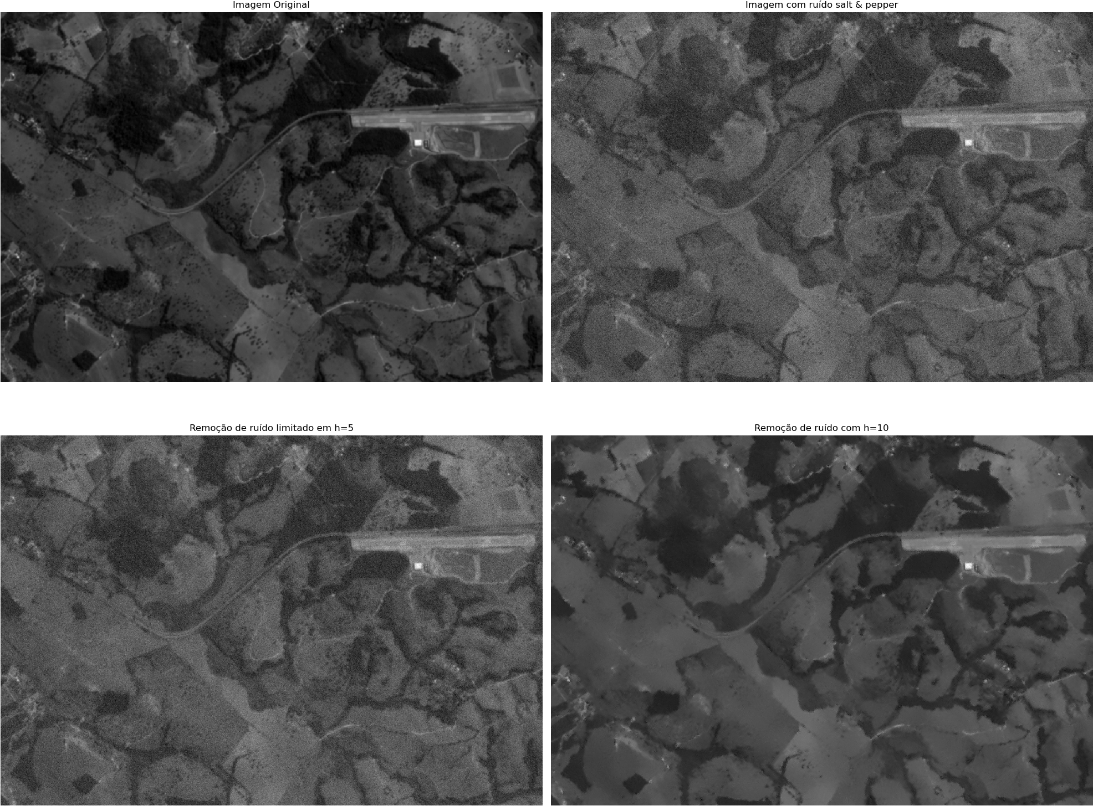
\includegraphics[width=0.8\columnwidth]{Figuras/res1-1.png}
		\end{figure}
	\end{frame}

	\begin{frame}{Resolução da Questão 1}
		\begin{figure}
			\centering
			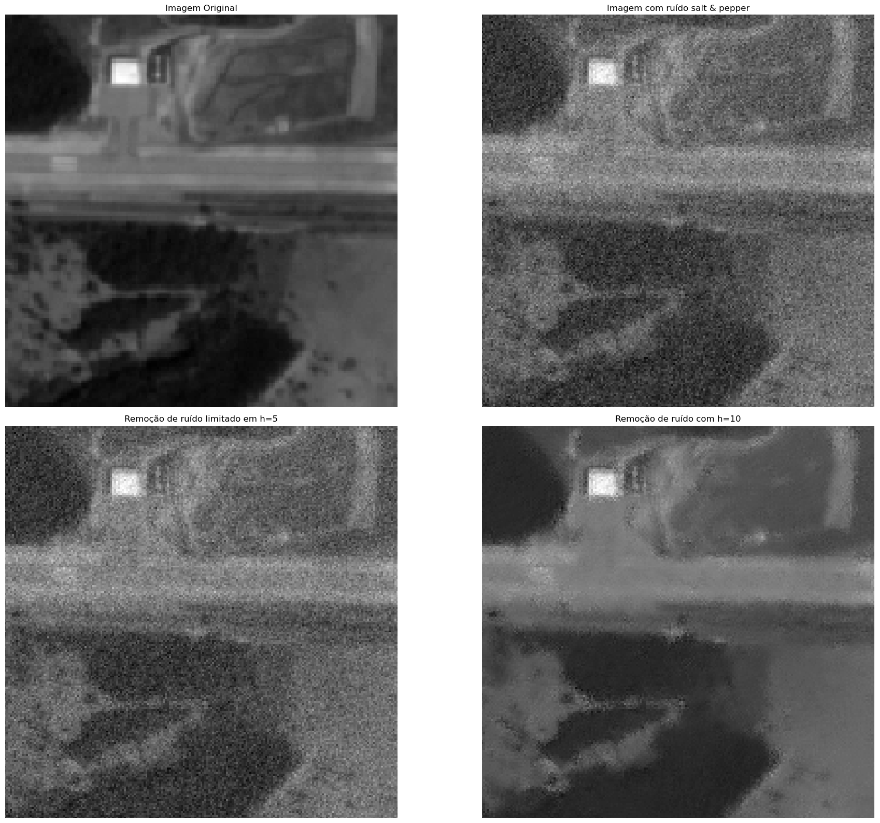
\includegraphics[width=0.7\columnwidth]{Figuras/res1-2.png}
		\end{figure}
	\end{frame}

	\subsection{Questão 2}
	\begin{frame}{Resolução da Questão 2}
		\begin{block}{Identificação de objeto}
			\textbf{Enunciado:} Implemente um código responsável pela seleção dos conjuntos de pixels associados à pista de aeroporto.
		\end{block}
		\begin{itemize}
			\item Com o OpenCV, foi possível identificar contornos na imagem e selecionar o contorno de maior área, correspondendo à pista de pouso.
		\end{itemize}
		\begin{figure}
			\centering
			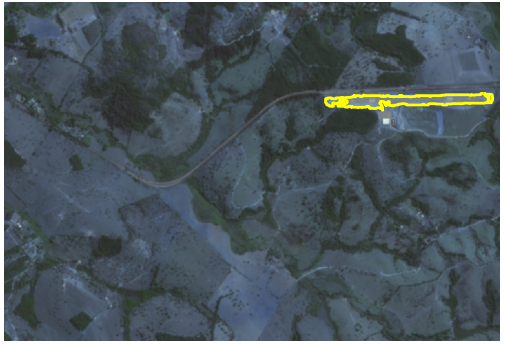
\includegraphics[width=0.6\columnwidth]{Figuras/res2-2.png}
		\end{figure}
	\end{frame}


	\begin{frame}{Resolução da Questão 2}
		\begin{block}{Identificação de vegetação em imagens de 8 bandas}
			\textbf{Enunciado:} Considerando um conjunto de imagens satelitais provenientes do sensor WorldView-2 (resolução de 0.5m e 8 bandas espectrais, em arquivos .tif), implemente algum método para segmentação da vegetação presente nas cenas.
		\end{block}
		\begin{itemize}
			\item De acordo com o artigo "High density biomass estimation for wetland vegetation using WorldView-2 imagery and random forest regression algorithm" disponível na pasta Referências, o índice NDVI (Normalized Difference Vegetation Index) é muito utilizado para identificar vegetação em imagens do WorldView-2.
			\item Para calcularmos o $NDVI = \frac{(NIR - Red)}{(NIR + Red)}$.
			\item Foi necessária a instalação da biblioteca tifffile para abrir as imagens TIFF.
		\end{itemize}
	\end{frame}

	
	\begin{frame}{Resolução da Questão 2}
		\begin{figure}
			\centering
			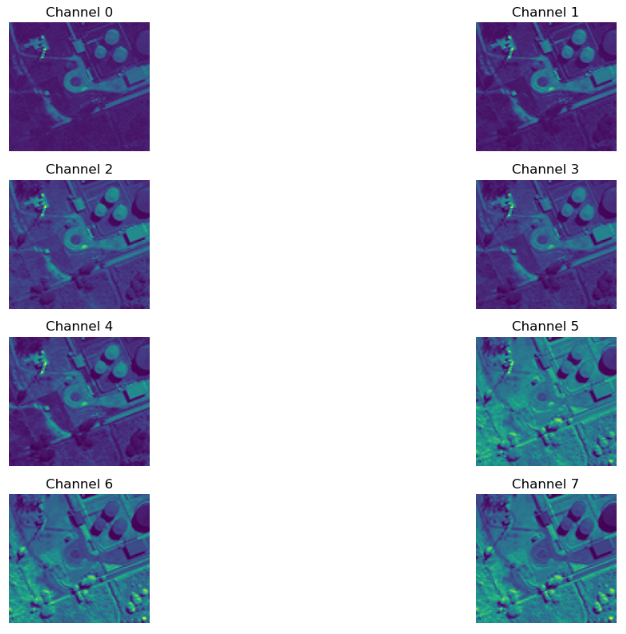
\includegraphics[width=0.66\columnwidth]{Figuras/res2-1.png}
		\end{figure}
	\end{frame}

	\begin{frame}{Resolução da Questão 2}
		\begin{itemize}
			\item A partir do cálculo do NDVI, foi possível identificar a vegetação presente na imagem de satélite.
		\end{itemize}
		\begin{columns}
			\begin{column}{0.5\linewidth}
				\begin{figure}
					\centering
					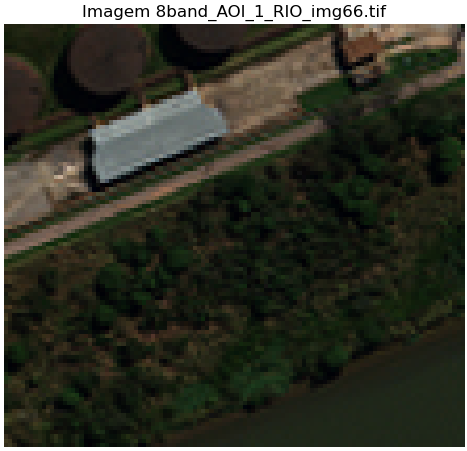
\includegraphics[width=0.9\columnwidth]{Figuras/res2-3.png}
				\end{figure}
			\end{column}
			\begin{column}{0.5\linewidth}
				\begin{figure}
					\centering
					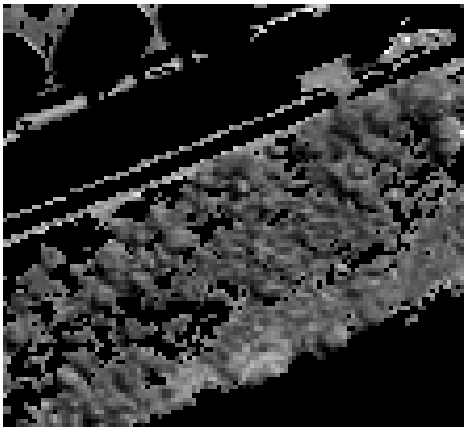
\includegraphics[width=0.9\columnwidth]{Figuras/res2-4.png}
				\end{figure}
			\end{column}
		\end{columns}
	\end{frame}


	\subsection{Questão 3}
	\begin{frame}{Resolução da Questão 3}
		\begin{block}{Segmentação}
			\textbf{Enunciado:} Seja o conjunto de dados associado à construções, sobre imagens satelitais, implemente algum modelo responsável pela segmentação das residências presentes nas imagens satelitais.
		\end{block}
		\begin{figure}
			\centering
			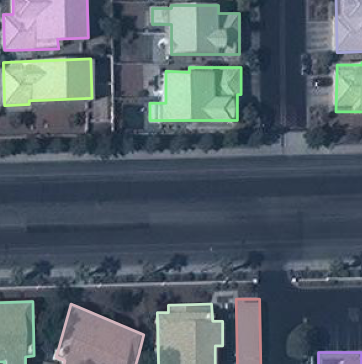
\includegraphics[width=0.45\columnwidth]{Figuras/res3-1.png}
		\end{figure}
	\end{frame}


	\begin{frame}{Resolução da Questão 3}
		\begin{itemize}
			\item Para solucionar este problema, utilizamos a biblioteca FastAI que facilita a implementação de \textbf{transfer learning}, agilizando muito o processo de treinar um modelo de segmentação.
			\item Foram utilizadas apenas 200 imagens do dataset para chegar a uma precisão aceitável, como pode ser verificado na imagem (Target/Prediction).
		\end{itemize}
		\begin{figure}
			\centering
			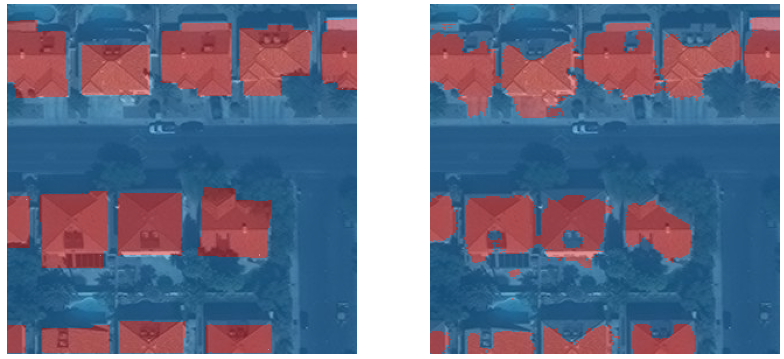
\includegraphics[width=0.8\columnwidth]{Figuras/res3-3.png}
		\end{figure}
	\end{frame}

	\section{Considerações Finais}
	\begin{frame}{Considerações Finais}
		\begin{itemize}
			\item Todos os três problemas foram solucionados com êxito.
			\item Os slides apresentados focaram nos resultados alcançados.
			\item Através dos notebooks disponibilizados no GitHub, é possível entender como os problemas foram solucionados. Além disso, também é possível reproduzir os resultados, visto que todas as configurações e instalações necessárias estão gravadas nos notebooks.
			\item Devido ao curto espaço de tempo, não foi possível incluir as soluções em Docker containers, sendo que possuo experiência com a utilização de Dockers.
		\end{itemize}
	\end{frame}
	
\end{document}